\onlyinsubfile{\setcounter{section}{3}}
\section{Results}
\label{sec:chapter2-results}

% Stata exports tabular-only bodies (no \begin{table}); this wrapper owns float, caption, label, notes, width.
\providecommand{\ChapterTableNoteText}[1]{\parbox[t]{0.94\textwidth}{#1}}
\providecommand{\InputStataRegTable}[4]{%
\begin{table}[htbp]
\centering
\caption{#1}%
\label{#2}%
\begin{threeparttable}
\small
\begin{adjustbox}{max width=\textwidth}
\input{#3}%
\end{adjustbox}
\begin{tablenotes}[flushleft]
\footnotesize
\item \ChapterTableNoteText{#4}%
\end{tablenotes}
\end{threeparttable}
\end{table}%
}
% Tighter layout for wide panel tables (e.g.\ RE/CRE with many footer rows).
\providecommand{\InputStataRegTableCompact}[4]{%
\begin{table}[htbp]
\centering
\caption{#1}%
\label{#2}%
\begin{threeparttable}
\begingroup
\footnotesize
\setlength{\tabcolsep}{4pt}%
\renewcommand{\arraystretch}{0.94}%
\begin{adjustbox}{max width=\textwidth}
\input{#3}%
\end{adjustbox}
\endgroup
\begin{tablenotes}[flushleft]
\footnotesize
\item \ChapterTableNoteText{#4}%
\end{tablenotes}
\end{threeparttable}
\end{table}%
}

%%%%%%%%%%%
\par The presence of hump-shaped empirical relationship between earnings and trust in the HRS data is important because it aligns with previous literature \cite{jbpglg2016}. Given the oversampling of older and retired households by the HRS, this is an important first step towards using the dataset to argue a similar pattern trust and returns.

\par I focus the statistical analysis on returns to net wealth only. \footnote{The results for the smaller portfolio compositions (core, retirement, residential, and core and retirement) are largely insignificant across specifications (though the results are more encouraging when retirement assets are excluded).} Again, with more retirees in the sample, an analysis of retirement assets may take more creative efforts. That said, I show that trust is predictive for the raw measure of returns to net wealth, and the relationship is robust to different trimming and winsorization choices. Due to the number of outliers in the sample, I present the results for a top and bottom winsorization of 5\% for returnns to net wealth. \footnote{This is important given the difficulty with computing returns in the U.S. due to lack of available data on flows in and out of narrowly defined asset classes.}


\subsection{Trust and average returns to net wealth}

\par I begin the analysis of the empirical relationship between the average returns to net wealth over the period 2002-2022 and the 2020 trust measure. This is captured by the regression equation \[\bar{r}^{net}_{i} = X_{i}'\beta + \varepsilon_{i}.\] Trust in ths model is assumed to be an invariant characteristic about households (measured in a single wave, but the same across waves) that influences economic decisions over time so that it matters for long-run returns. \footnote{\cite{Lesmeister2019} is an example of work which also assumes trust is time invariant.}

\InputStataRegTableCompact{\textbf{Trust and Average Returns to Net Wealth}}{tab:38_avg_returns}{../../Code/Analysis/Tables/38_table1_avg_returns.tex}{OLS. Heteroskedasticity-robust standard errors. Columns \textit{(3)--(4)} add wealth deciles, age bins, labor force, and education; column \textit{(4)} adds gender, race, region, immigration status, and marital status.}
\FloatBarrier

\par First, allowing for the hump-shaped relationship between trust and returns by adding the quadratic term for trust not only increases the predictive power of returns, but considerably increases the explained variation of the model. Second, as for other variables which reject the null hypothesis of no significant effect on returns, wealth and age add the most to explained variation, followed by labor force participation status and years of education. These controls represent the minimal, baseline specification of the model, captured by column 3 in the table. ~\ref{tab:38_avg_returns}. A final specifcation, with additional demographic variables, is robust to the hump-shaped relationship, as well as the predictive power of labor force participation status for returns.\footnote{As we will see later, Race and Gender are variables which predict trust well, so they are additional demographic variables which may be of interest here.}

\subsection{Pooled regression model}

\par With the implicit assumption that the 2020 trust measure is constant for respondents, then the hump-shaped relationship holds between trust and long-run, average returns to net wealth in the HRS data. A key object of analysis in the empirical heterogeneous returns literature is the estimated persistent component of returns. To build toward this, we move to the panel regression model \[r^{net}_{it} = \lambda_t + X_{it}'\beta + \varepsilon_{it}.\] In table ~\ref{tab:38_pooled}, I  show that the hump-shaped relationship persists in the pooled baseline model and with the maximal set of controls.

\InputStataRegTableCompact{\textbf{Pooled OLS of Returns to Net Wealth on Trust}}{tab:38_pooled}{../../Code/Analysis/Tables/38_table2_pooled.tex}{Person-year OLS. Standard errors clustered by household. Column \textit{(1)}: baseline controls (wealth, age, labor force, education, year effects). Column \textit{(2)}: adds gender, race, region, immigration status, and marital status.}
\FloatBarrier

\par Interestingly, not only do the variables in the minimal set of controls (wealth, age, labor force participation, education), but the year dummies, race, gender, and marital status all show significant predictive power for returns to net wealth in the pooled regression. Furthermore, adding the full set of controls increases the (unadjusted) R-squared by almost one-fourth.

\subsection{Panel regression models}

\subsubsection{The Fixed Effects (FE) model}

\par The next step is to allow for individual fixed effects in the panel regression so that the error term $\varepsilon_{it}$ can be written as \[\varepsilon_{it} = \alpha_{it} + e_{it},\] where $e_{it}$ may possibly be serially correlated. Notably, the predictive power of any the time-invariant regressors (trust, education, race, gender, region, immigration status) will be absored by the individual fixed effect term. Table~\ref{tab:38_fe_1st} reports two within-household specifications that differ only in which \emph{time-varying} controls are added on top of the same wealth-decile indicators, five-year age-bin fixed effects, and survey-year fixed effects (those blocks enter both columns but are summarized by joint tests in the lower panel rather than coefficient-by-coefficient). Column~\textit{(1)} isolates labor-force participation as the only time-varying demographic shown in the body of the table. Column~\textit{(2)} adds marital status and wave-specific census region (relative to Northeast), with the joint tests for marital status and region reported alongside the tests for age bins, wealth deciles, and years.

\InputStataRegTableCompact{\textbf{Panel OLS with Individual Fixed Effects}}{tab:38_fe_1st}{../../Code/Analysis/Tables/38_table3a_fe_1st.tex}{Within (household) fixed-effects estimator. Standard errors clustered by household. Time-invariant regressors absorbed. Column~\textit{(1)}: wealth deciles, age-bins, labor force, and year FE. Column~\textit{(2)}: Additional controls include time-varying marital status and census region. Reported $\rho$, $\sigma_u$, and $\sigma_e$ are variance-component estimates from the FE decomposition.}
\FloatBarrier

\par The parameters $\rho$, $\sigma_u$, and $\sigma_e$ are of particular interest, as they summarize the variance decomposition of the error term in the panel regression. In this framework, $\sigma_u$ denotes the standard deviation of the unobserved individual-specific component, $\alpha_i$, capturing persistent differences in returns across individuals. The parameter $\sigma_e$ is the standard deviation of the idiosyncratic error term, $\varepsilon_{it}$, reflecting within-individual variation over time that is not explained by the included covariates.

\par The parameter $\rho$ represents the fraction of the total variance attributable to the individual-specific component, defined as
\[
\rho = \frac{\sigma_u^2}{\sigma_u^2 + \sigma_e^2}.
\]
A high value of $\rho$ indicates that a substantial share of the variation in returns arises from persistent differences across individuals, providing evidence of heterogeneity in returns across respondents.

\par The within-$R^2$ measures the proportion of within-individual variation in returns explained by the time-varying regressors---how much of the deviation of an individual's returns from their own mean is accounted for by observables.

\par Focus on the second column of Table~\ref{tab:38_fe_1st}. There remains substantial within-person variation not captured by time-varying regressors $\sigma_e^2(=.33)$. Heterogeneity across individuals captured by $\sigma_u^2(=.45)$ is larger than in the RE or CRE specifications reported below, which explains why $\rho$ is much higher here ($\rho=.65$). The within-$R^2$ in that column is $(=.18)$. Because time-invariant regressors are absorbed by the household fixed effects, the estimated individual-specific component captures persistent heterogeneity across households, including variation that would otherwise load on time-invariant observables.

\par Figure~\ref{fig:37_fe_hist} shows the distribution of estimated fixed effects from the column~\textit{(2)} first-stage FE specification (the same extended time-varying controls as in that column), analogous to how Figure~\ref{fig:37_cre_hist} reports the CRE individual effect when time-invariant controls are included. In this setting, where time-invariant factors like education and trust are absorbed, the estimated distribution is particularly comparable to empirical estimates of the same object using Norwegian population data from 2004-2015 by \cite{aflgdmlp20} and using the PSID from 1999-2019 by \cite{Daminato2024}.

\begin{figure}[htbp]
  \centering
  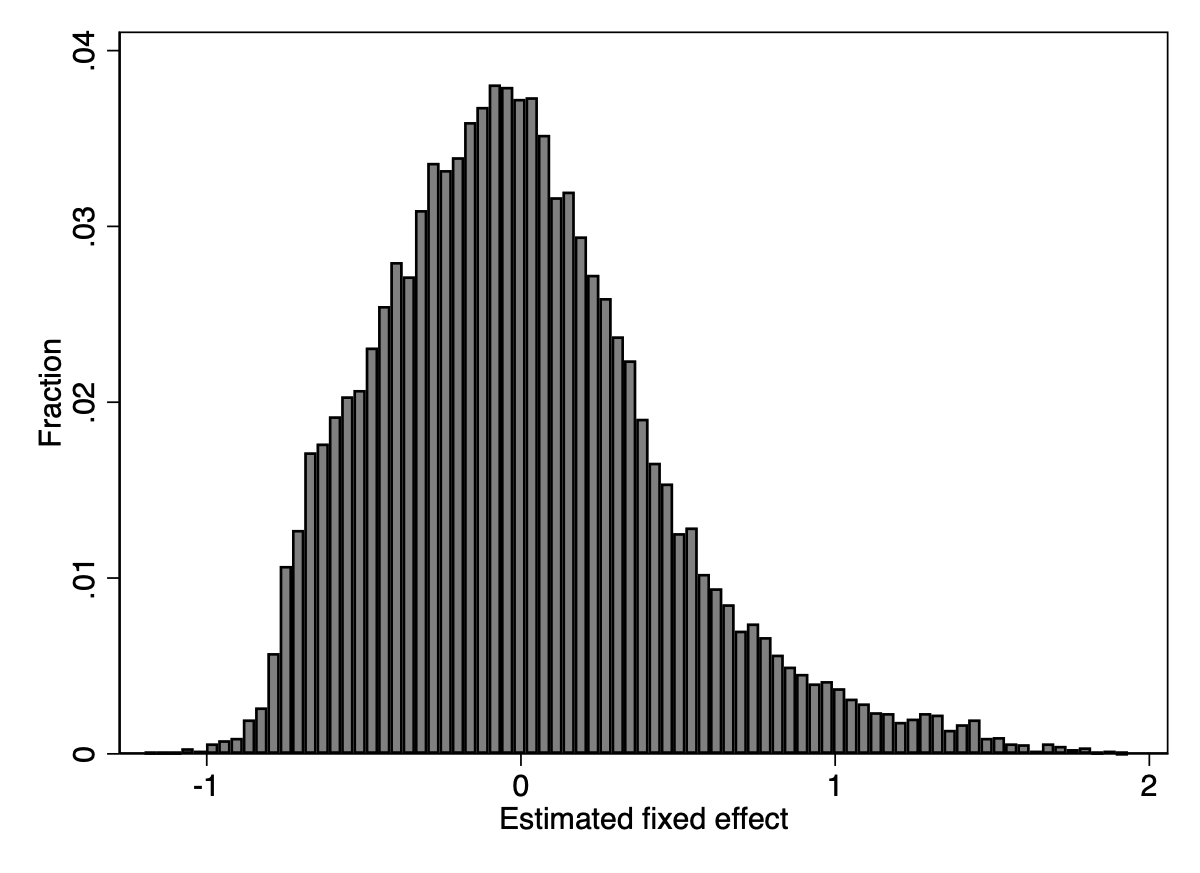
\includegraphics[width=0.8\textwidth]{../../Code/Analysis/Figures/37_fe_hist.png}
  \caption{Distribution of estimated fixed effect (FE) with extended set of controls.}
  \label{fig:37_fe_hist}
\end{figure}
\FloatBarrier

\par Figure~\ref{fig:43_fe_vs_wpct_37} shows that the estimated household fixed effect is strongly \emph{downward} sloping in wealth percentile. A direct check in Stata reproduces this pattern: the correlation between the predicted fixed effect and wealth percentile is about $-0.778$, and the slope from a simple regression of the predicted fixed effect on wealth percentile is about $-0.0138$ ($p<0.001$). This should not be read as saying that wealth lowers raw returns. Rather, the fixed effect here is the residual household-specific intercept left after removing time-varying variation associated with wealth deciles, age bins, labor-force status, year effects, and in the extended specification marital status and region.

\begin{figure}[htbp]
  \centering
  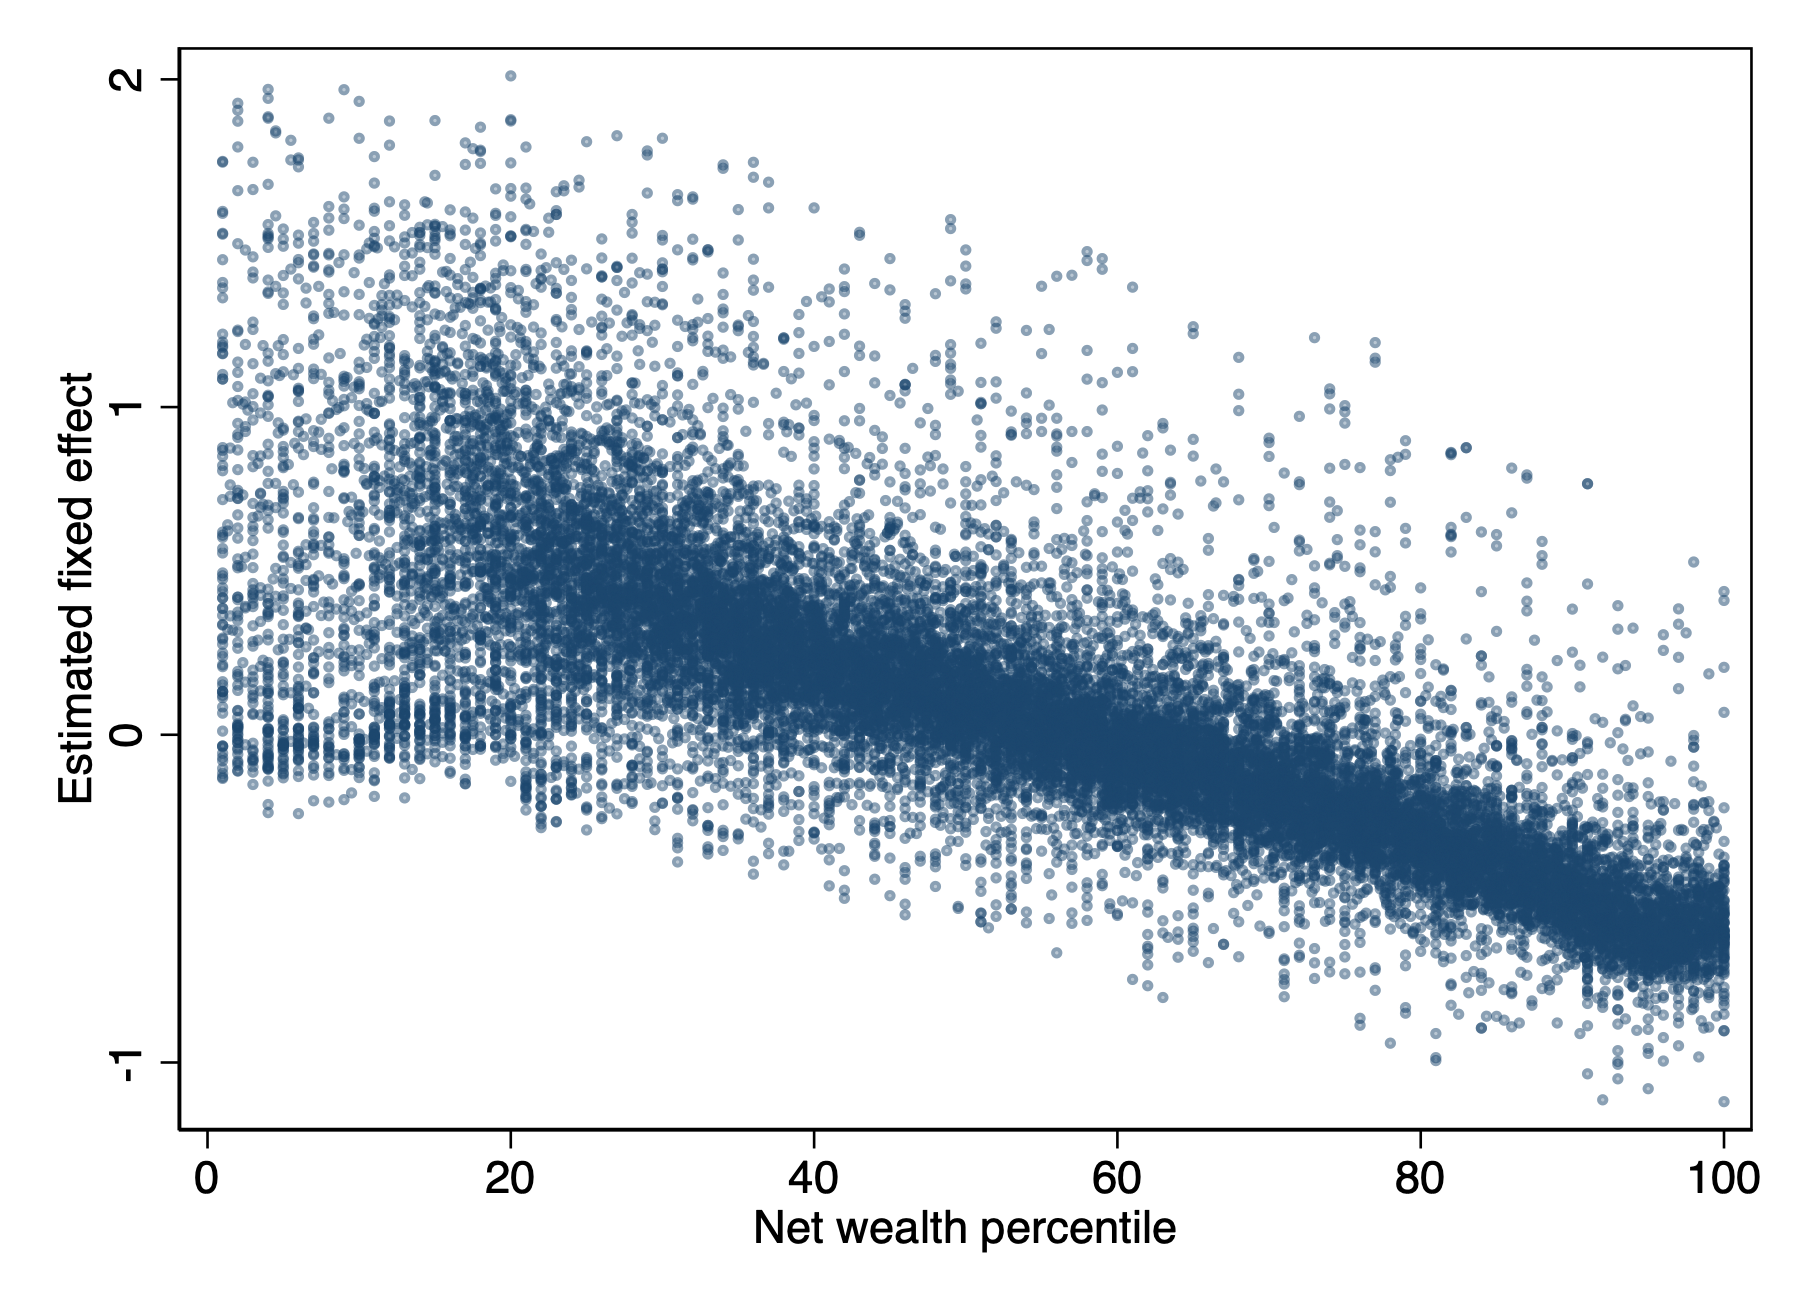
\includegraphics[width=0.8\textwidth]{../../Code/Analysis/Figures/43_fe_vs_wpct_37.png}
  \caption{Estimated fixed effect vs.\ net wealth percentile (extended controls).}
  \label{fig:43_fe_vs_wpct_37}
\end{figure}
\FloatBarrier

\par It is a bit unsavory to show that a suite of factors, including the hump-shaped trust relationship, matter for explaining the variation in trust, but then to exclude them when characterizing the persistent component of returns. Said differently, we would like to control for these differences when describing how individuals differ in their returns on average.

\par To move in this direction, I begin by regressing the estimated fixed effect onto the time-invariant variables which were excluded from the regression once the indivdiual fixed effect was accounted for in the model. In table ~\ref{tab:38_fe_2nd}, race and education seem to have the most predictive power regarding variation in the predicted individual effects. The negative education coefficients are not a coding mistake: they are reproduced even in a simple cross-sectional regression of the predicted fixed effect on $i.educ\_cat$, and they become more negative at higher education categories. At the same time, I hesitate to give these signs a strong structural interpretation. The left-hand side in this second-stage regression is itself a generated regressor from the first-stage FE model, so the coefficients should be read as descriptive correlations with the estimated residual household intercept after the first stage has already removed time-varying variation.

\InputStataRegTableCompact{\textbf{Explaining Estimated Fixed Effect with Time-Invariant Controls}}{tab:38_fe_2nd}{../../Code/Analysis/Tables/38_table3_fe_2nd.tex}{Cross-sectional OLS of predicted household fixed effects on time-invariant regressors. Heteroskedasticity-robust standard errors. The dependent variable in column~\textit{(1)} is the fixed effect from the Table~\ref{tab:38_fe_1st} column~\textit{(1)} specification; in column~\textit{(2)} it is the fixed effect from column~\textit{(2)} of that table (so time-varying marital status and census region are already part of the first-stage FE when forming the left-hand side). Column~\textit{(1)}: education categories and trust; column~\textit{(2)}: adds gender, race/ethnicity, US-born, and census region.}
\FloatBarrier

\subsubsection{The Random Effects (RE) model}

\par The model with fixed effects is one specification of the general panel regression model, when the term capturing the latent time-invariant variation affecting returns for individuals $\alpha_i$ is possibly correlated with the observable, time-varying variables $X_{it}$. The Random Effects (RE) model allows for estimation and inference in a similar setting by assuming that the $\alpha_i$'s are normally distributed with some constant variance, but that $Cov(\alpha_i, X_{it}) = 0$.

\par Since it is not clear that this persistent component capturing differences in returns is uncorrelated with factors like wealth, age, and labor force particiaption, this is an assumption which should be tested to determine if the RE model is the right one for empirical relationship between trust and returns that we are after. The p-value for the test-statistic with controls ($p<.01$) and without controls ($p<.01$) strongly reject that the estimated coeffients are efficeint under the RE model. This suggests that it is not preferred over the standard fixed effects model, with all time-invariant explanatory power captured by $\alpha_i$.

\par That said, one can still describe the variance structure of the estimated fixed effect in the RE setting. Focus on the second column of Table~\ref{tab:38_re}. There is significant within-person variation not captured by time-varying regressors $\sigma_e^2(=.36)$. However, the estimates of heterogeneity across individuals captured by $\sigma_u^2$ is much smaller here $(=.18)$. These two features combined explains why the value for $\rho$ is much closer to $0$ here than in the FE model. That said, a value of $\rho=.20$ still represents substaintial heterogeneity.

\InputStataRegTableCompact{\textbf{The RE Model for Trust and Returns to Net Wealth}}{tab:38_re}{../../Code/Analysis/Tables/38_table4_re.tex}{Random-effects GLS. Standard errors clustered by household. Within $R^2$ reported. $\rho$, $\sigma_u$, and $\sigma_e$ are variance-component estimates from the RE decomposition. Joint tests are Wald tests for the indicated covariate blocks.}
\FloatBarrier

\subsubsection{The Correlated Random Effects (CRE) model}

\par The rejection of the RE model is informative, but it does not help with the issue that we would like to account for the variation of time-invariant factors (like education and trust) while still characterizing the persistent component of returns for individuals. To do so, we move to the Correlated Random Effects (CRE) model, where the assumption of is $Cov(\alpha_i, X_{it}) = 0$ relaxed; the persistent component and time-varying factors are allowed to be correlated. 

\par First, recall that the FE model is equivalent to demeaning within individuals:\footnote{In the empirical implementation below, the correlated random-effects specification is estimated manually using the traditional Mundlak device rather than Stata 19's dedicated \texttt{xtreg, cre} syntax. Concretely, I estimate \texttt{xtreg, re} and augment the right-hand side with respondent-level means of the time-varying regressors, which is the same econometric construction that earlier Stata workflows required users to code by hand before Stata 19 automated it and paired it with \texttt{estat mundlak}. The panel used in file 38 is strongly balanced, despite the legacy dataset name, so the within-respondent means of the survey-year indicators are constants across households. For that reason, I do not add averages of the year dummies separately in the Mundlak augmentation: in this balanced-panel setting they are collinear with the intercept and add no identifying variation.}
\[
r^{net}_{it} = \alpha_i + \lambda_t + X_{it}'\beta + \varepsilon_{it},
\]

\par For each individual $i$, take the time average:
\[
\bar{r}^{net}_i = \alpha_i + \bar{\lambda}_i + \bar{X}_i'\beta + \bar{\varepsilon}_i,
\]

\par Then subtract from the original equation:
\[
r^{net}_{it} - \bar{r}^{net}_i
=
\left(\lambda_t - \bar{\lambda}_i\right)
+ \left(X_{it} - \bar{X}_i\right)'\beta
+ \left(\varepsilon_{it} - \bar{\varepsilon}_i\right),
\]

\par Notice that the individual fixed effect is eliminated by this transformation. As a result, any time-invariant regressors are also removed from the model.

\par The correlated random effects (CRE) model instead augments the regression with the individual-specific means of the time-varying regressors:
\[
r^{net}_{it}
=
\alpha_i + \lambda_t + X_{it}'\beta + \bar{X}_i'\theta + \varepsilon_{it},
\]

\par where $\bar{X}_i$ denotes the within-individual averages of the regressors. The term $\bar{X}_i'\theta$ explicitly captures the correlation between the unobserved individual component $\alpha_i$ and the observed variables $X_{i,t}$. In the manual implementation used here, the reported Mundlak test is the cluster-robust Wald test that the coefficients on all added respondent-level mean terms are jointly zero, which is the manual equivalent of Stata 19's \texttt{estat mundlak}. That null is overwhelmingly rejected in both CRE specifications, with $p \approx 8.0\times 10^{-44}$ in the baseline column and $p \approx 1.8\times 10^{-43}$ in the extended column, strongly favoring the CRE specification over standard RE. The key finding of this paper is that, \textit{the coefficeints on the trust coefficients are statistically significant in the CRE setting, where the persistent component of returns can be estimated as well}. This can be seen in Table ~\ref{tab:38_cre}.

\InputStataRegTableCompact{\textbf{The CRE (Mundlak) Model for Trust and Returns to Net Wealth}}{tab:38_cre}{../../Code/Analysis/Tables/38_table5_cre.tex}{Random effects with respondent-level Mundlak means of the time-varying regressors. Standard errors clustered by household. Within $R^2$ reported. $\rho$, $\sigma_u$, and $\sigma_e$ are variance-component estimates from the RE decomposition of the augmented CRE specification. ``Mundlak test $p$'' reports the cluster-robust Wald test of the null that the coefficients on all added panel means are jointly zero, the manual equivalent of Stata 19's \texttt{estat mundlak}.}
\FloatBarrier

\par With the estimated individual fixed effect being a key empirical object of this paper, the interpretation of the variance structure is important here. Focus on the second column of Table~\ref{tab:38_cre}. Much like the FE and RE models, there is significant within-person variation not captured by time-varying regressors $\sigma_e^2(=.36)$. Moreover, the estimates of heterogeneity across individuals captured by $\sigma_u^2$ are smallest here $(=.15)$. These two features combined explains why the value for $\rho=.15$, documenting significant cross-sectional variation.

\par Figure~\ref{fig:37_cre_hist} shows the distribution of the estimated CRE individual effect from the specification when controls are included. The estimated distribution is comparable estimated the using Norwegian population data and using the PSID, though less so than the FE model (especially near the center of the distriution).

\begin{figure}[htbp]
  \centering
  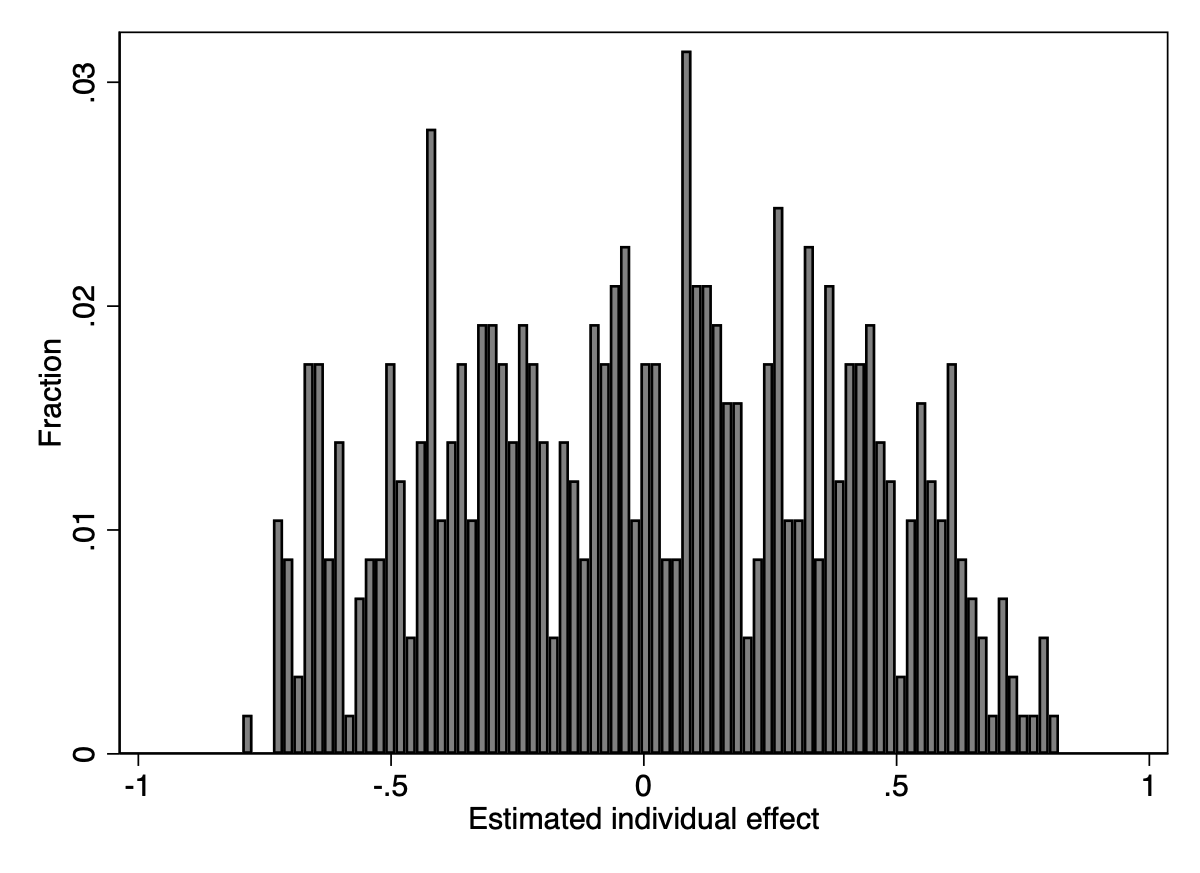
\includegraphics[width=0.8\textwidth]{../../Code/Analysis/Figures/37_cre_hist.png}
  \caption{Distribution of Estimated Fixed Effect (CRE) with extended set of controls..}
  \label{fig:37_cre_hist}
\end{figure}
\FloatBarrier

\begin{figure}[htbp]
  \centering
  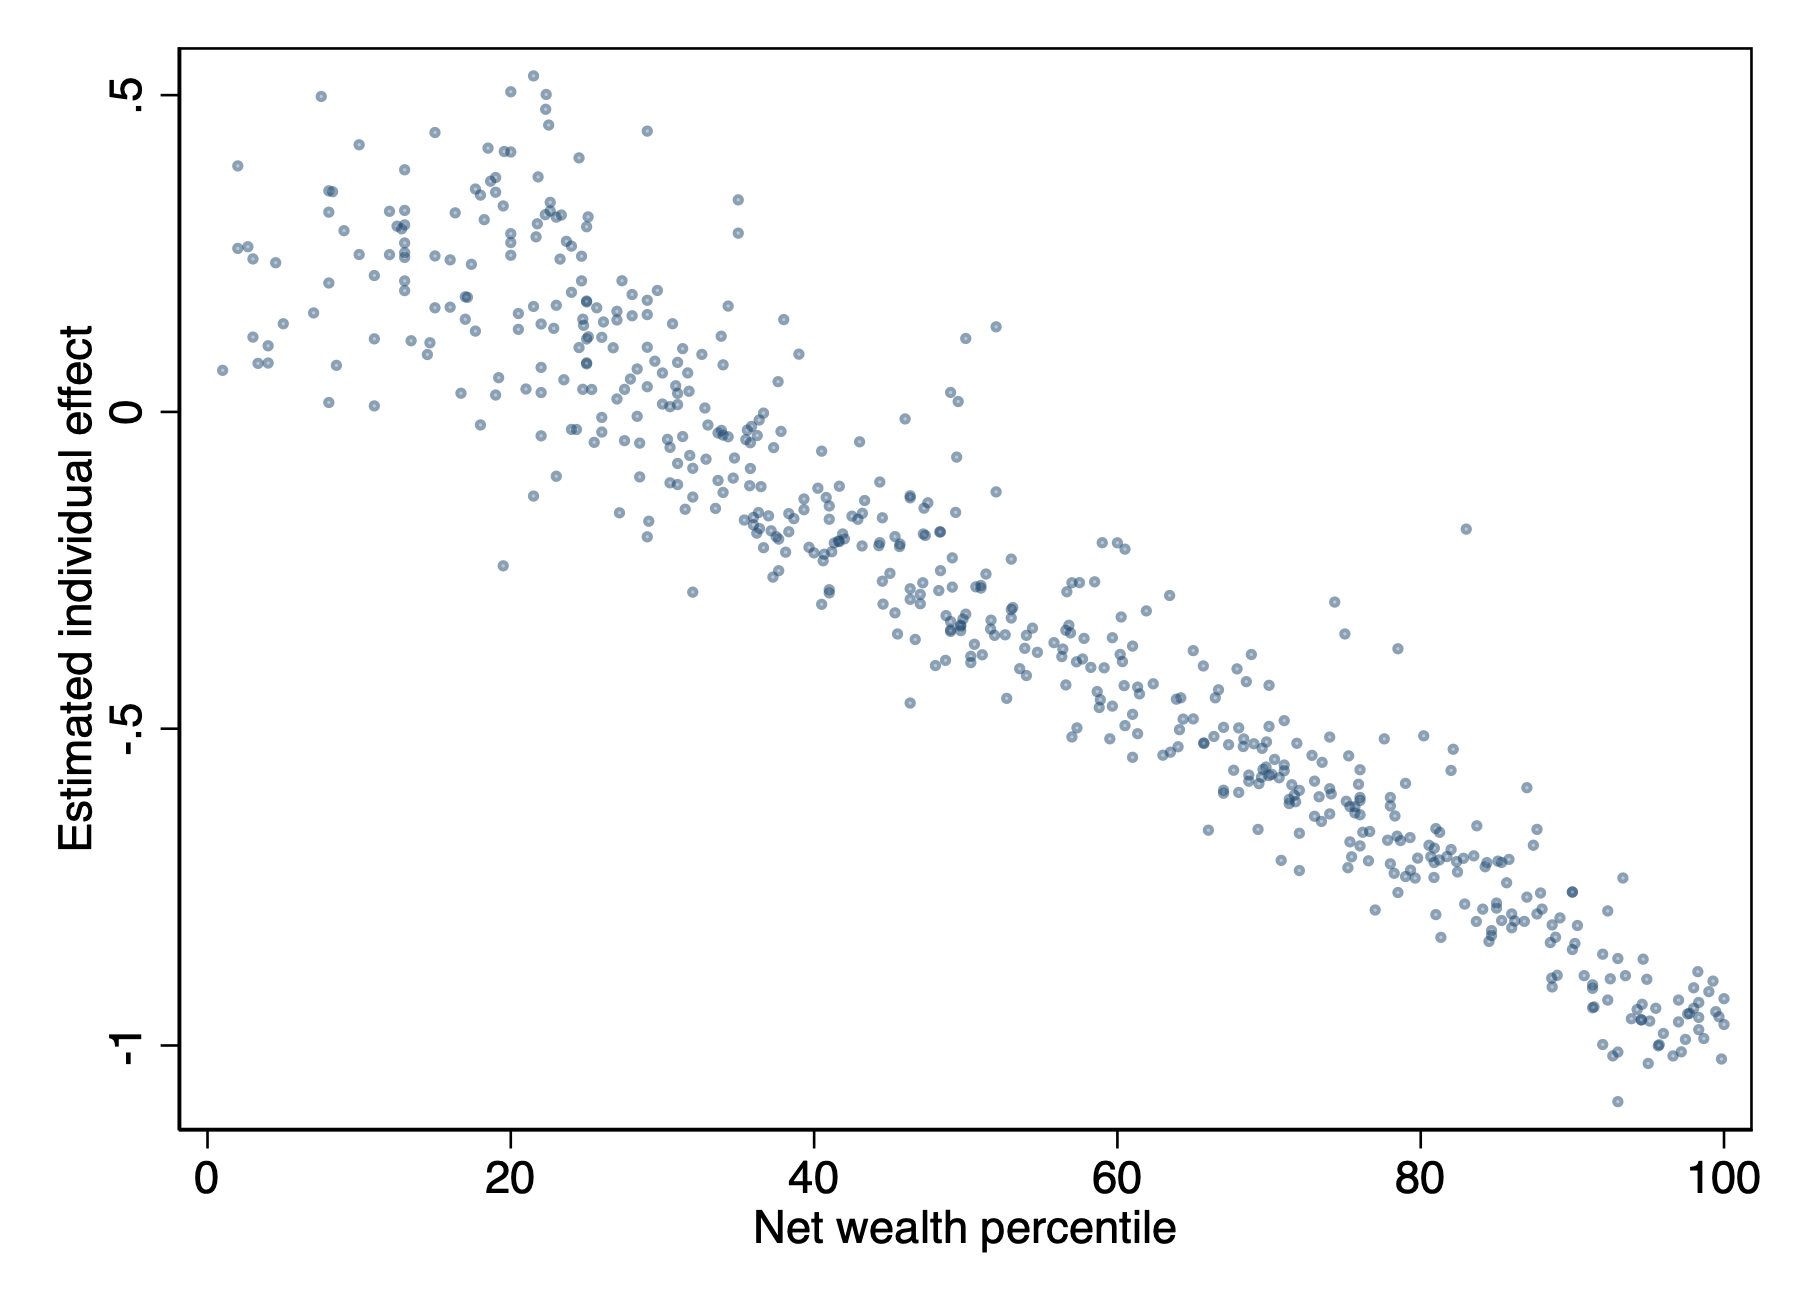
\includegraphics[width=0.8\textwidth]{../../Code/Analysis/Figures/43_cre_vs_wpct_37.png}
  \caption{Estimated CRE individual effect vs.\ net wealth percentile (extended controls).}
  \label{fig:43_cre_vs_wpct_37}
\end{figure}
\FloatBarrier

\par Figure~\ref{fig:43_cre_vs_wpct_37} shows the same basic pattern for the CRE individual effect. The relationship is again downward sloping, though flatter than in the FE case. The interpretation is the same as above: this figure is about the estimated residual persistent component after accounting for observed time-varying covariates and, in the CRE specification, their respondent-level means. It should therefore not be read as the raw relationship between returns and wealth, which is shown earlier in Figure~\ref{fig:39_r5_netwealth_pct}.

\subsection{Which level of trust maximizes returns?}

\par By choosing to model the hump-shaped relationship between trust and returns using a combination of a linear and quadratic terms, I can describe the level of trust which maximizes returns to net wealth in the following way. Starting from
\[
r^{net}_{it} = \alpha_i + \lambda_t + X_{it}'\beta + \varepsilon_{it},
\]
 holding controls fixed, the implied marginal effect of trust is
\[
\frac{\partial r^{net}_{it}}{\partial \textit{Trust}_i} = \beta_1 + 2\beta_2 \textit{Trust}_i.
\]
Setting this derivative to zero gives the critical point $\textit{Trust}^* = -\beta_1/(2\beta_2)$. When $\hat\beta_1 \geq 0$ and $\hat\beta_2 \leq 0$, the fitted relationship in trust is concave (hump-shaped), and the estimated trust level that maximizes fitted returns to net wealth is $\textit{Trust}^* = -\hat\beta_1/(2\hat\beta_2)$, reported as $(\textit{Trust})^*$ in the Table~\ref{tab:38_trust_star}.

\InputStataRegTableCompact{\textbf{The Level of Trust which Maximizes Returns}}{tab:38_trust_star}{../../Code/Analysis/Tables/38_table6_trust_star.tex}{Panel A: minimal time-invariant controls (education only in panel specifications). Panel B: full demographics. Trust$^*$ computed as $-\hat\beta_1/(2\hat\beta_2)$; standard errors, $p$-values for $H_0\!:\mathrm{Trust}^*=0$, and 95\% confidence intervals use the delta method (\texttt{nlcom} in Stata). ``Both sig?'' indicates both trust terms significant at 10\% in separate tests; joint test is Wald on both trust terms.}
\FloatBarrier

\par In general, the level of trust which maxmimizes returns to net wealth is between $6$ and $7$. When controls are added, the maximal level of trust is generally higher than when controls are excluded for each regression model tested. Because \(\textit{Trust}^*\) is a nonlinear function of \(\hat\beta_1\) and \(\hat\beta_2\), Stata uses the delta method to approximate its standard error. I use this to report the standard error on the estimated maximal level of trust, as well as $95\%$ confidence intervals, and p-values which test \(H_0: \textit{Trust}^* = 0\).
